\documentclass[11pt]{article}
\usepackage{tocloft}
\usepackage{graphicx}
\usepackage{calc}
\usepackage{amssymb}
\usepackage{color}
\usepackage{array}
\usepackage[sc]{mathpazo}
\usepackage{url}
\usepackage[final]{pdfpages}

%\linespread{1.05}
\oddsidemargin=0pt
\evensidemargin=0pt
\textwidth=6.5in
\topmargin=0pt
\headheight=0pt
\headsep=0pt
\textheight=9in
% EXPERIMENTAL
%\parindent=0pt
%\parskip=3pt
\setlength{\parindent}{0cm}
\newcommand\secfont{\fontfamily{cmss}\selectfont}%\textwidth 5.5truein
\newcommand\pifheading[1]{{\secfont\textbf{#1}:}}
%\oddsidemargin -0.40truein
%\textheight 8.0truein
%\topmargin -0.25truein
\def\lo{
\mathrel{\raise.3ex\hbox{$<$}\mkern-14mu\lower0.6ex\hbox{$\sim$}}
}
\def\hi{
\mathrel{\raise.3ex\hbox{$>$}\mkern-14mu\lower0.6ex\hbox{$\sim$}}
}

\textwidth = 6.6 in
\textheight = 9.1 in
\oddsidemargin = -0.05 in
\evensidemargin = +0.05 in
\topmargin = -.1 in
\headheight = 0.0 in
\headsep = 0.0 in
\parskip = 0.06in
\newcommand\registered{{\ooalign{\hfil\raise .00ex\hbox{\scriptsize R}\hfil\crcr\mathhexbox20D}}}

%% Define a new 'leo' style for the package that will use a smaller font.
\makeatletter
\def\url@leostyle{%
  \@ifundefined{selectfont}{\def\UrlFont{\sf}}{\def\UrlFont{\small\ttfamily}}}
\makeatother
%% Now actually use the newly defined style.
\urlstyle{leostyle}

%\pagestyle{empty}
%\includeonly{previous,proposal_references}
%\includeonly{proposal_references}
%\includeonly{previous}

% TOC
\pagenumbering{gobble}
\begin{document}
%%%%%%%%%%%%%%%%%%%%%%%%%%%%%%%%%%%%%%%%%%%%%%%%%%%%%%%%%%%%%%%%%%%%%
\begin{center}
\textbf{\Large
AST101: Our Corner of the Universe \\
\vspace*{0.1cm}
Lab 3: Phases of the Moon Prelab
}
\end{center}

\vspace*{0.5cm}

\hrule
{\Large Name:}\vspace*{0.5cm}\\\hrule
{\Large Student number (SUID):}\vspace*{0.5cm}\\\hrule
{\Large Lab section:}\vspace*{0.5cm}\\\hrule
\vspace*{0.5cm}

%%%%%%%%%%%%%%%%%%%%%%%%%%%%%%%%%%%%%%%%%%%%%%%%%%%%%%%%%%%%%%%%%%%%%
\section{Introduction}

Please note that prelabs must be completed \underline{\textbf{before}} you arrive at your lab section, and your TA will verify that you have done so. If you have not completed your prelab before arriving you will be asked to leave, and will need to either complete your prelab in time to begin your lab, or find a different section. If you do neither, you will receive a zero for the lab.

\subsection*{Objective}

In this lab, we'll be working through some exercises involving predicting phases of the moon and what time of day the moon 
rises and sets. In the prelab, we want you to become familiar with the diagrams we'll use to reason through this.

Don't be discouraged by the large number of pages here; most of them are diagrams for you to fill out.

\subsection*{Basic ideas}

\begin{enumerate}
\item The Moon travels around the Earth about once every 27 days (about every four weeks).
\item The Sun always lights up half of the Moon -- the half that faces the Sun.
\item From Earth, we can only see half of the Moon -- the half that faces the Earth.
\item Since the Moon does not make its own light, we can only see the parts of the Moon that are illuminated by the Sun. Parts of the Moon that are not lit by the Sun are (almost) invisible.
\item What phase of the Moon we see is determined by {\bf what portion of the half we can see is illuminated by the Sun}.
\item Both the Earth and the Moon are small enough that the Moon's shadow does not usually fall on the Earth, and the Earth's
shadow usually does not fall on the Moon. When this happens, it is called an {\it eclipse}, and it happens only rarely and very 
briefly. {\it This is not what causes the phases of the moon.}
\end{enumerate}

\newpage
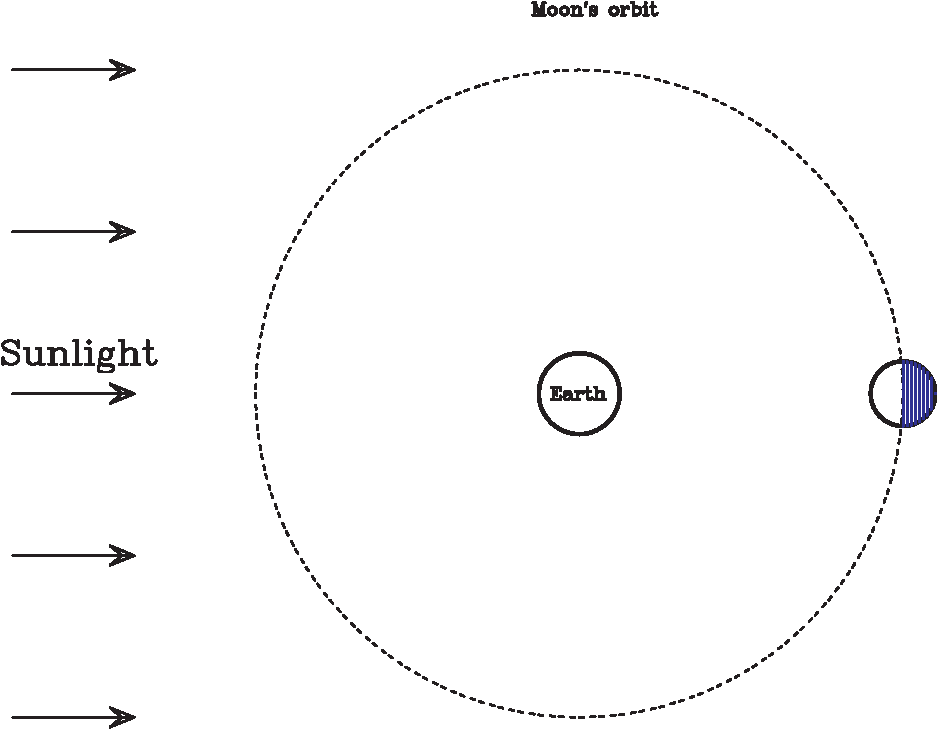
\includegraphics[width=0.8\textwidth]{moon-diagram-full-crop.pdf}


	The figure above shows the Moon in one possible place in its orbit around Earth. Notice that the left half of the Moon is
	bright since it is facing the Sun, and the right half of the Moon is dark, since it is facing away from the Sun. This is the same mechanism that causes night and day on Earth.

{\it 1. Which portion of the Moon can be seen from Earth? }

\vspace{0.8in}

{\it 2. Of the portion of the Moon that can be seen from Earth, how much is lit by the Sun?}

\vspace{0.8in}

{\it 3. What will the Moon look like? Either describe it in words, name the phase of the Moon, or draw it below.}
	
	\vspace{1.2in}
	
{\it 4. What time of day will this Moon be highest in the sky?}
\newpage

\newpage
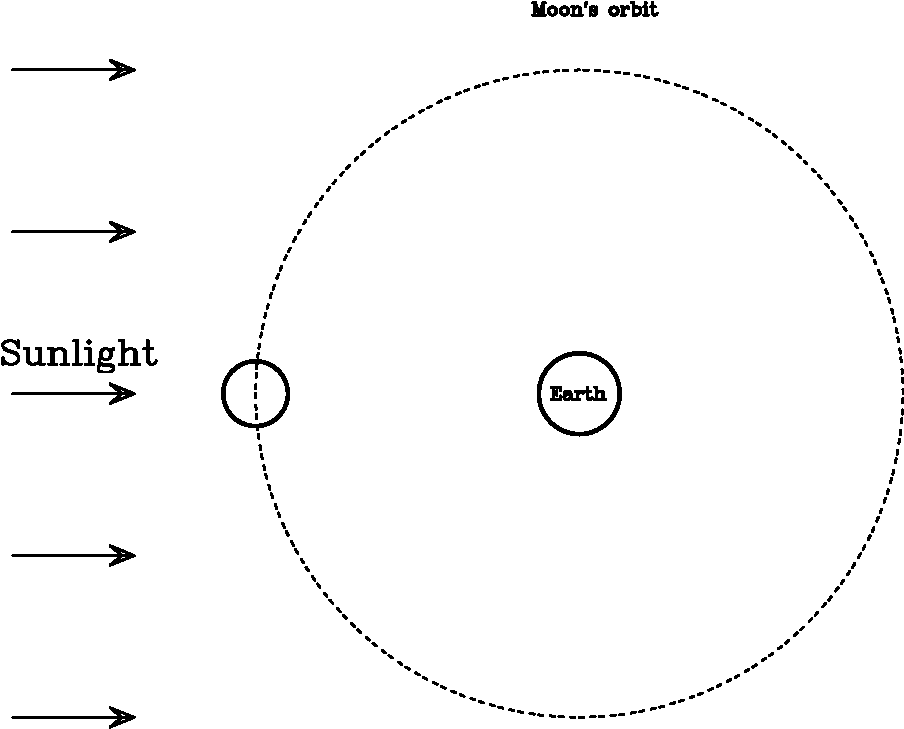
\includegraphics[width=0.8\textwidth]{moon-diagram-new-crop.pdf}


The figure above shows the Moon in a different place in its orbit.

{\it 5. Shade in the portion of the Moon that is lit by the Sun.}

{\it 6. Which portion of the Moon can be seen from Earth? }

\vspace{0.9in}

{\it 7. Of the portion of the Moon that can be seen from Earth, how much is lit by the Sun?}

\vspace{0.9in}

{\it 8. What will the Moon look like now?}

\vspace{1.8in}

\newpage

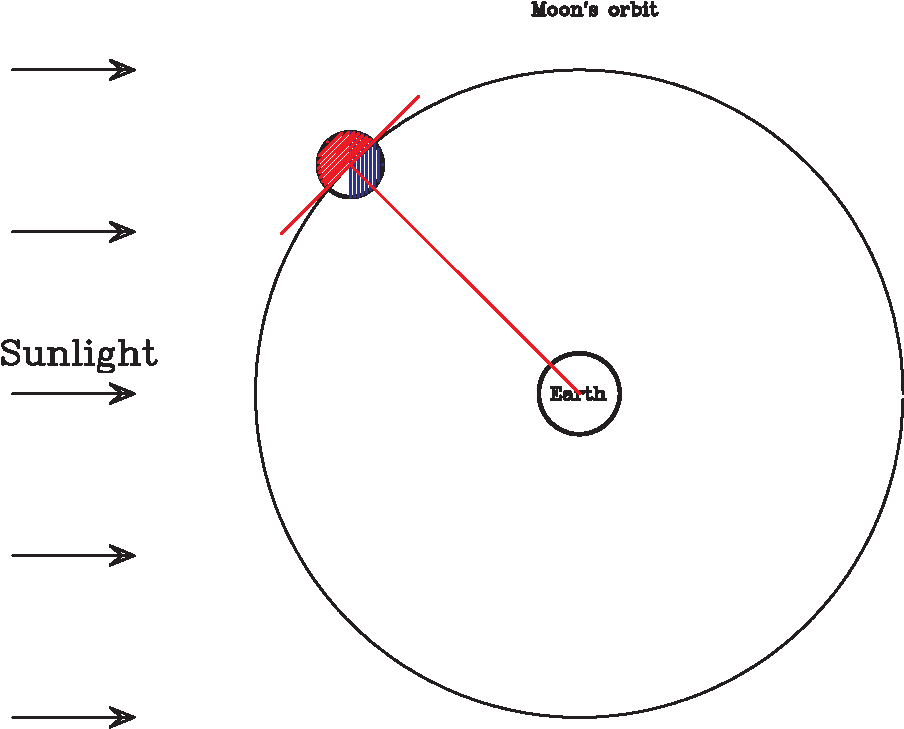
\includegraphics[width=0.8\textwidth]{moon-diagram-crescent-crop.pdf}

Here is another diagram. This time I have drawn a line from the Earth's center to the Moon's center, then drawn another line from Earth to the Moon. Note that:

\begin{itemize}
	\item The right half of the Moon is shaded blue: this is the part that you can't see, because it's not lit by the Sun
	\item The top-left half of the Moon, shaded in red, is the part that can't be seen from Earth because it is facing away from Earth.
	\item Here, {\it most} of the half of the Moon that is facing Earth is also {\it not} lit by the Sun.
	\item The only part of the Moon that is {\it facing Earth} and also {\it lit by the Sun} is the piece that is not shaded in red or in blue -- the bottom-left portion.
	\item Since only a small piece of the side of the Moon facing Earth is lit by the Sun, we will only see a small part of the disk of the Moon: a crescent.
\end{itemize}

{\it 9. Will this Moon mostly be above the horizon during the day or during the night?}

\newpage
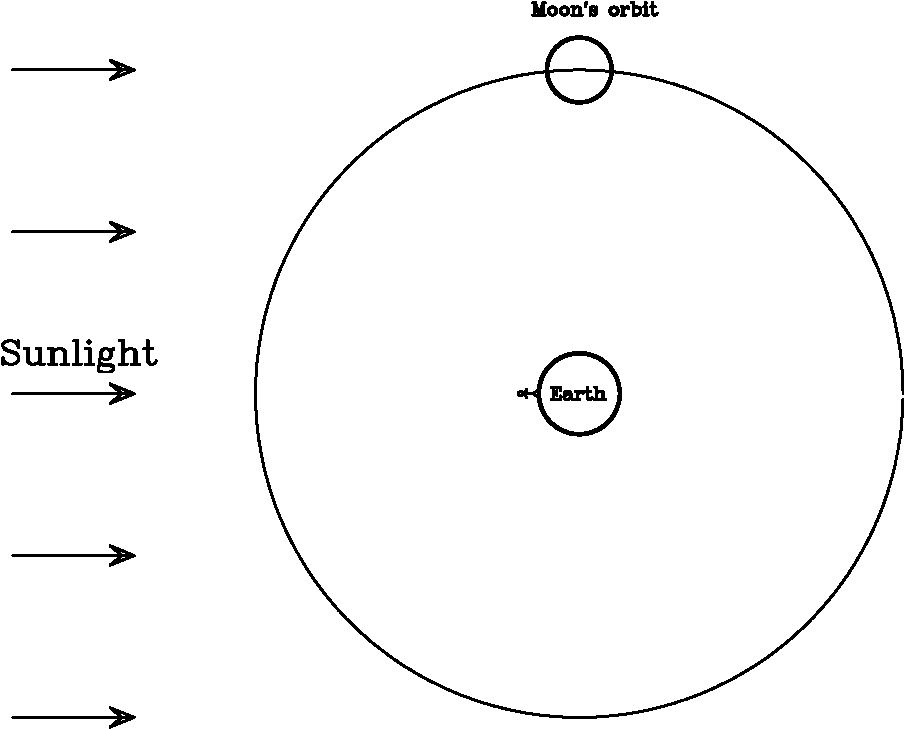
\includegraphics[width=0.8\textwidth]{moon-diagram-half-crop.pdf}

Here's one more diagram. 

{\it 10. Shade in the portion of the Moon that is not lit by the Sun (and thus invisible)}

{\it 11. Draw a line from the Earth to the Moon, and then draw another line perpendicular to it that cuts the Moon in half. Shade in the half that we can't see because it is facing away from Earth.}

{\it 12. What fraction of the part of the Moon that is facing Earth is lit by the Sun? What will this Moon look like?}

\vspace{1.5in}

{\it 13. Where will the observer shown here see the Moon in their sky? (Will it be high in the sky, or low on the horizon? You'll learn how to figure out which horizon is which in the actual lab.}



\end{document}
